%! TeX program = lualatex
\documentclass[a4paper]{article} 

% packages
\usepackage{microtype}      % Slightly tweak font spacing for aesthetics
\usepackage[english]{babel} % Language hyphenation and typographical rules
\usepackage[final, colorlinks = true, urlcolor = black, linkcolor = black]{hyperref} 
\usepackage{changepage}     % adjust margins on the fly

\usepackage{fontspec}
\setmainfont{EB Garamond}
\setmonofont[Scale=MatchLowercase]{Deja Vu Sans Mono}

\usepackage{minted}
\usemintedstyle{algol_nu}
\usepackage{xcolor}

\usepackage{pgfplots}
\pgfplotsset{width=\textwidth,compat=1.9}

\usepackage{caption}
\newenvironment{code}{\captionsetup{type=listing}}{}
\captionsetup[listing]{skip=0pt}
\setlength{\abovecaptionskip}{5pt}
\setlength{\belowcaptionskip}{5pt}

\usepackage[yyyymmdd]{datetime}
\renewcommand{\dateseparator}{--}

\usepackage{titlesec}
% \titleformat{\section}{\LARGE\bfseries}{}{}{}[\titlerule]
% \titleformat{\subsection}{\Large\bfseries}{}{0em}{}
% \titlespacing{\subsection}{0em}{-0.7em}{0em}
%
% \titleformat{\subsubsection}{\large\bfseries}{}{0em}{$\bullet$ }
% \titlespacing{\subsubsection}{1em}{-0.7em}{0em}

% margins
\addtolength{\hoffset}{-2.25cm}
\addtolength{\textwidth}{4.5cm}
\addtolength{\voffset}{-3.25cm}
\addtolength{\textheight}{5cm}
\setlength{\parskip}{0pt}
\setlength{\parindent}{0in}
% \setcounter{secnumdepth}{0}

\begin{document}
\hrule \medskip
\begin{minipage}{0.295\textwidth} 
    \raggedright
    \footnotesize 
    \begin{tabular}{@{}l l}
        Name: & Andrew Hayes \\
        Student ID: & 21321503 \\
        E-mail: & \href{mailto://a.hayes18@universityofgalway.ie}{a.hayes18@universityofgalway.ie} \\
    \end{tabular}
\end{minipage}
\begin{minipage}{0.4\textwidth} 
    \centering 
    \vspace{0.4em}
    \LARGE
    \textsc{ct404} \\ 
\end{minipage}
\begin{minipage}{0.295\textwidth} 
    \raggedleft
    \today
\end{minipage}
\medskip\hrule 
\begin{center}
    \normalsize
    Assignment 2: Image Processing \& Analysis
\end{center}
\hrule

\section{A Morphological Image Processing Pipeline for Medical Images}
\begin{figure}[H]
    \centering
    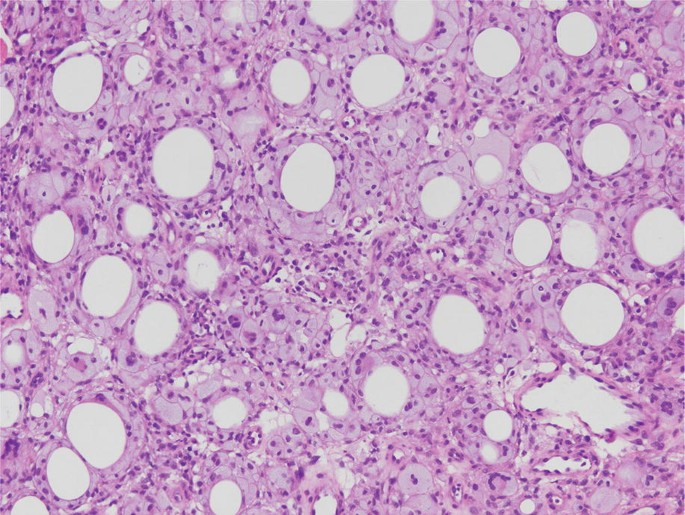
\includegraphics[width=0.7\textwidth]{../Task1.jpg}
    \caption{Original Skin Biopsy Image}
\end{figure}

\subsection{Conversion to A Single-Channel Image}
\begin{code}
\inputminted[linenos, breaklines, frame=single]{python}{../code/task1/1_single_channel_conversion.py}
\caption{\mintinline{python}{1_single_channel_conversion.py}}
\end{code}

Since the image has predominant hues of pink-purple, we would expect the green-channel-only image to be the one that yields the highest contrast, as pink \& purple colours are made up primarily by the blue \& red channels: the dominance of these channels results in little variance in intensity within these channels, and therefore green will have the highest intensity variance.
This is proven true by the text output of the above code, where the standard deviation of the greyscale image based off the green channel alone is by far the highest:
\begin{figure}[H]
    \centering
    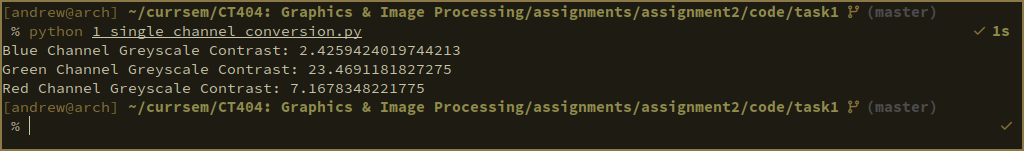
\includegraphics[width=\textwidth]{./images/1_single_channel_conversion_output.png}
    \caption{Output of \mintinline{python}{1_single_channel_conversion.py}}
\end{figure}

\noindent
\begin{minipage}{0.24\textwidth}
    \centering
    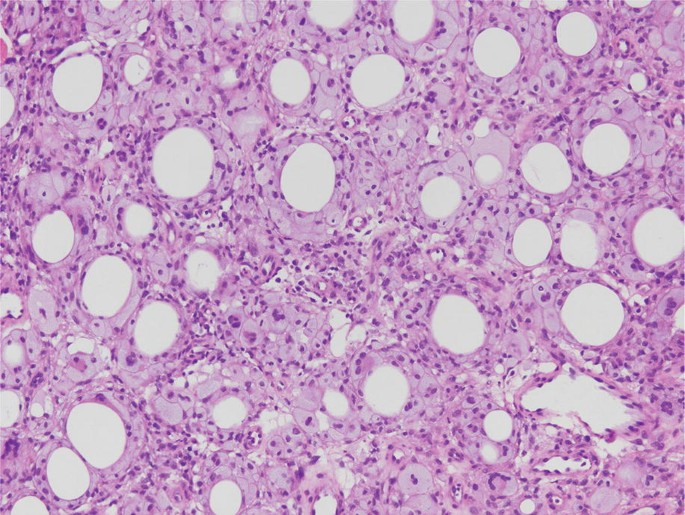
\includegraphics[width=\textwidth]{../Task1.jpg}
    \captionof{figure}{Original image}
    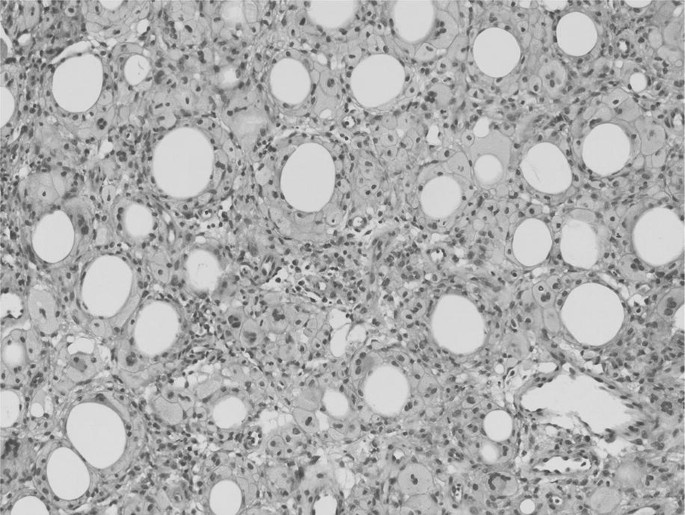
\includegraphics[width=\textwidth]{../code/task1/output/greyscale.jpg}
    \captionof{figure}{Greyscale original}
\end{minipage}
\hfill
\begin{minipage}{0.24\textwidth}
    \centering
    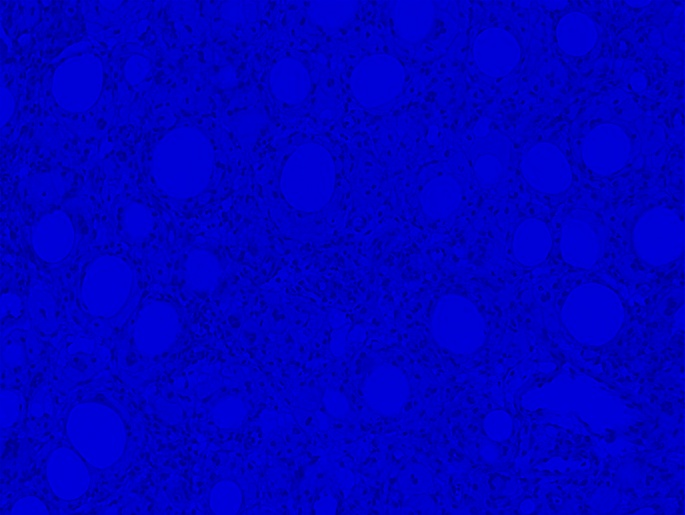
\includegraphics[width=\textwidth]{../code/task1/output/b_channel.jpg}
    \captionof{figure}{B-Channel}
    
\includegraphics[width=\textwidth]{../code/task1/output/b_channel_greyscale.jpg}
    \captionof{figure}{B-Greyscale}
\end{minipage}
\hfill
\begin{minipage}{0.24\textwidth}
    \centering
    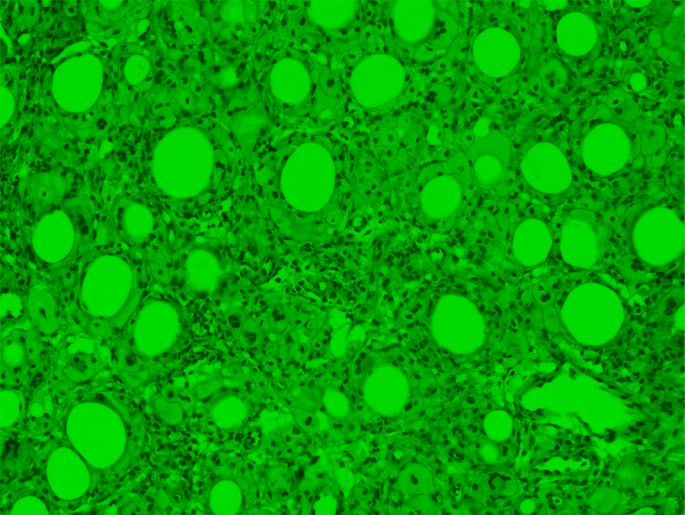
\includegraphics[width=\textwidth]{../code/task1/output/g_channel.jpg}
    \captionof{figure}{G-Channel}
    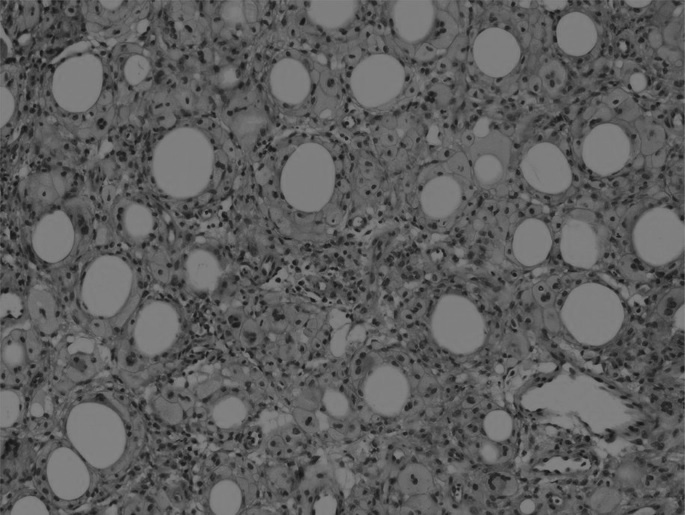
\includegraphics[width=\textwidth]{../code/task1/output/g_channel_greyscale.jpg}
    \captionof{figure}{G-Greyscale}
\end{minipage}
\hfill
\begin{minipage}{0.24\textwidth}
    \centering
    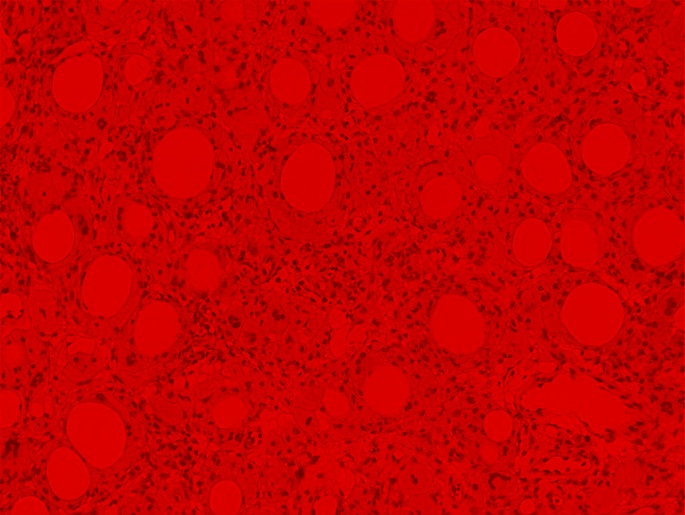
\includegraphics[width=\textwidth]{../code/task1/output/r_channel.jpg}
    \captionof{figure}{R-Channel}
    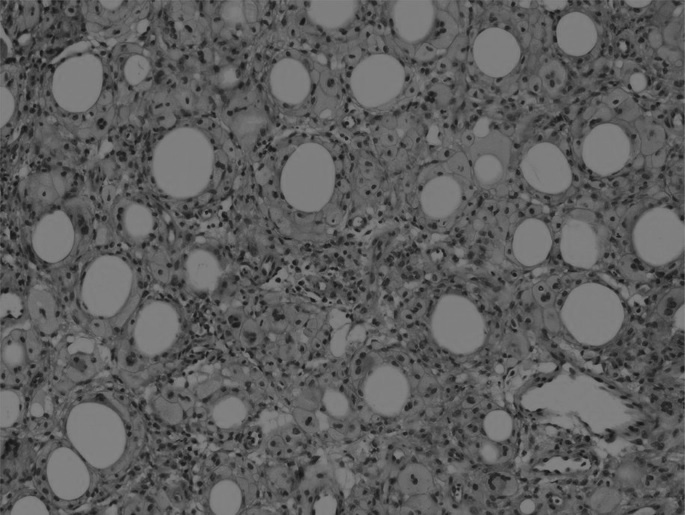
\includegraphics[width=\textwidth]{../code/task1/output/r_channel_greyscale.jpg}
    \captionof{figure}{R-Greyscale}
\end{minipage}

My selected single-channel image is the greyscale version of the green-channel-only image, as it yields the greatest contrast:
\begin{figure}[H]
    \centering
    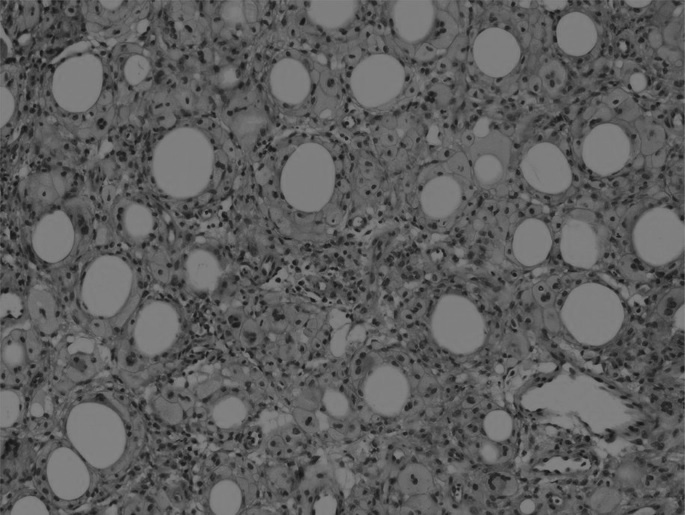
\includegraphics[width=0.5\textwidth]{../code/task1/output/g_channel_greyscale.jpg}
    \caption{Selected single-channel image: greyscale green-channel-only}
\end{figure}

\subsection{Image Enhancement}
\begin{code}
\inputminted[linenos, breaklines, frame=single]{python}{../code/task1/2_image_enhancement.py}
\caption{\mintinline{python}{2_image_enhancement.py}}
\end{code}

\begin{figure}[H]
    \centering
    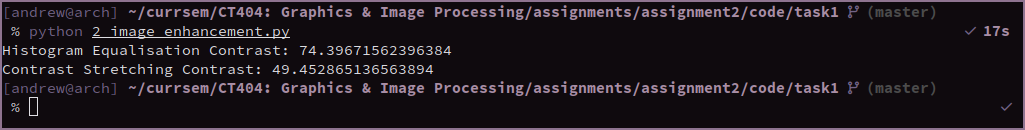
\includegraphics[width=\textwidth]{./images/2_image_enhancement_output.png}
    \caption{Output of \mintinline{python}{2_image_enhancement.py}}
\end{figure}

I chose to use the histogram equalisation technique as it gave the best contrast, as seen from the calculated standard deviation in contrast above and in the output images below.

\begin{minipage}{0.49\textwidth}
    \centering
    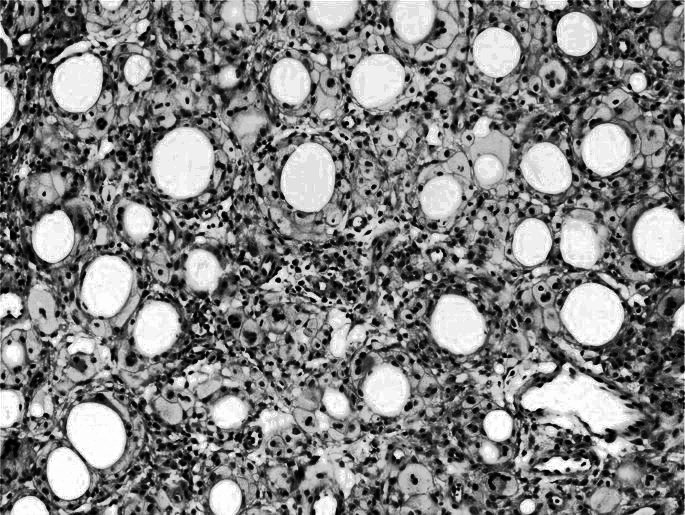
\includegraphics[width=\textwidth]{../code/task1/output/histogram_equalised.jpg}
    \captionof{figure}{Histogram-equalised image}
\end{minipage}
\hfill
\begin{minipage}{0.49\textwidth}
    \centering
    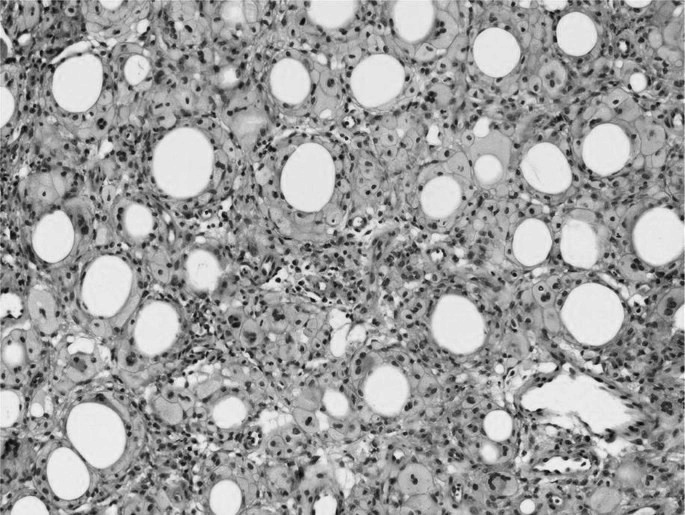
\includegraphics[width=\textwidth]{../code/task1/output/contrast_stretched.jpg}
    \captionof{figure}{Contrast-stretched image}
\end{minipage}

\subsection{Thresholding}
\begin{code}
\inputminted[linenos, breaklines, frame=single]{python}{../code/task1/3_thresholding.py}
\caption{\mintinline{python}{3_thresholding.py}}
\end{code}

\begin{figure}[H]
    \centering
    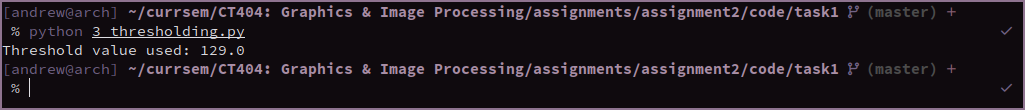
\includegraphics[width=\textwidth]{./images/3_thresholding_output.png}
    \caption{Output of \mintinline{python}{3_thresholding.py}}
\end{figure}

I used Otsu's algorithm to find the optimal threshold value that best separated the foreground (objects of interest) from the background.
As can be seen from the above output, the optimal value chosen was 129.

\begin{figure}[H]
    \centering
    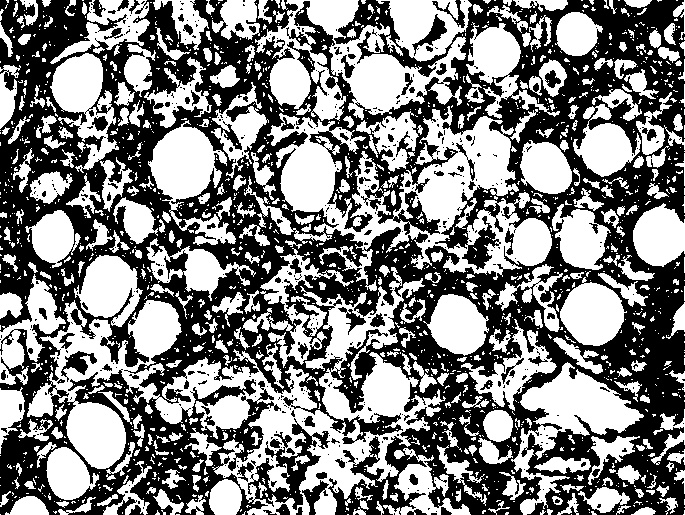
\includegraphics[width=0.5\textwidth]{../code/task1/output/otsu.jpg}
    \caption{Image with Otsu thresholding}
\end{figure}


\subsection{Noise Removal}
\begin{code}
    \inputminted[linenos, breaklines, frame=single]{python}{../code/task1/4_noise_removal.py}
    \caption{\mintinline{python}{4_noise_removal.py}}
\end{code}

\noindent
\begin{minipage}{0.24\textwidth}
    \centering
    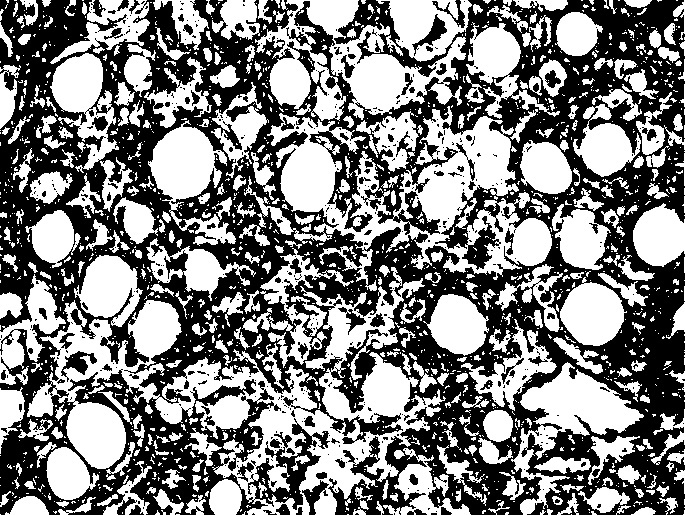
\includegraphics[width=\textwidth]{../code/task1/output/kernel_size_1.jpg}
    \captionof{figure}{\mintinline{python}{kernel_size = 1}}
\end{minipage}
\hfill
\begin{minipage}{0.24\textwidth}
    \centering
    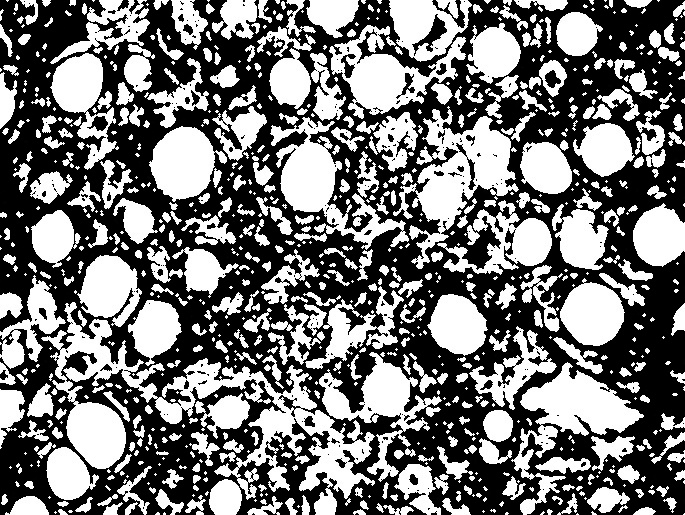
\includegraphics[width=\textwidth]{../code/task1/output/kernel_size_3.jpg}
    \captionof{figure}{\mintinline{python}{kernel_size = 3}}
\end{minipage}
\hfill
\begin{minipage}{0.24\textwidth}
    \centering
    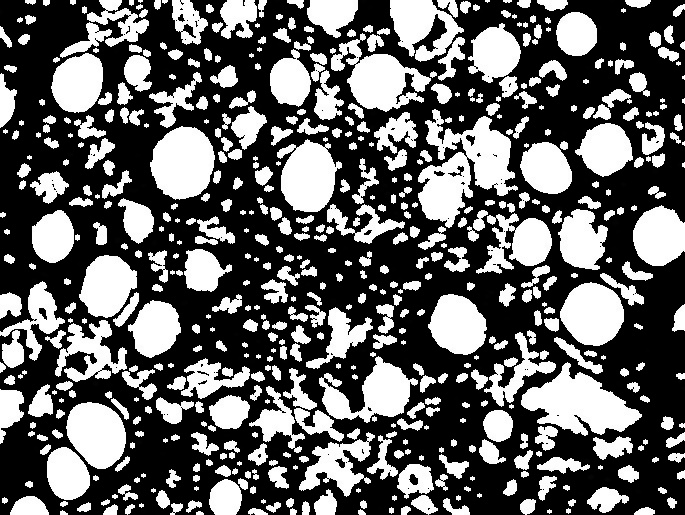
\includegraphics[width=\textwidth]{../code/task1/output/kernel_size_5.jpg}
    \captionof{figure}{\mintinline{python}{kernel_size = 5}}
\end{minipage}
\hfill
\begin{minipage}{0.24\textwidth}
    \centering
    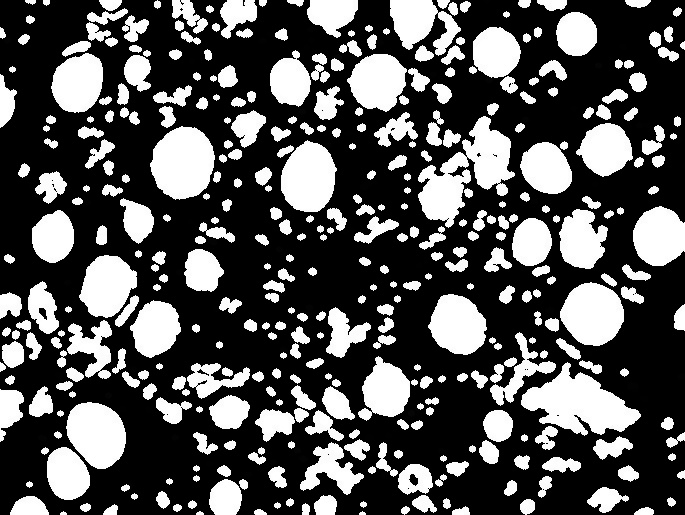
\includegraphics[width=\textwidth]{../code/task1/output/kernel_size_7.jpg}
    \captionof{figure}{\mintinline{python}{kernel_size = 7}}
\end{minipage}

\begin{minipage}{0.24\textwidth}
    \centering
    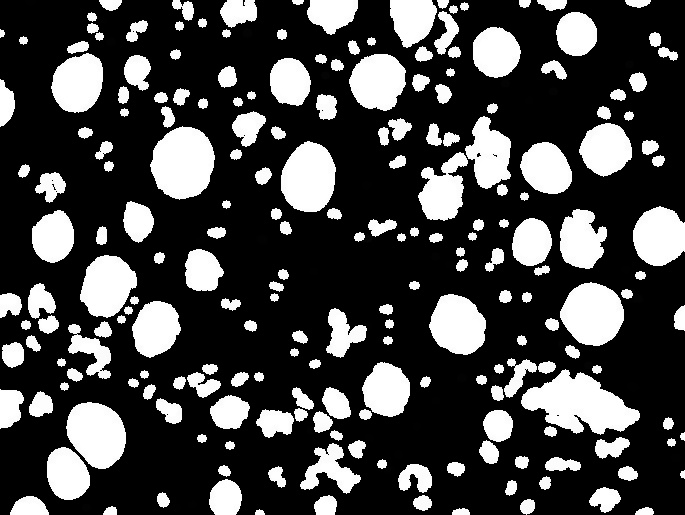
\includegraphics[width=\textwidth]{../code/task1/output/kernel_size_9.jpg}
    \captionof{figure}{\mintinline{python}{kernel_size = 9}}
\end{minipage}
\hfill
\begin{minipage}{0.24\textwidth}
    \centering
    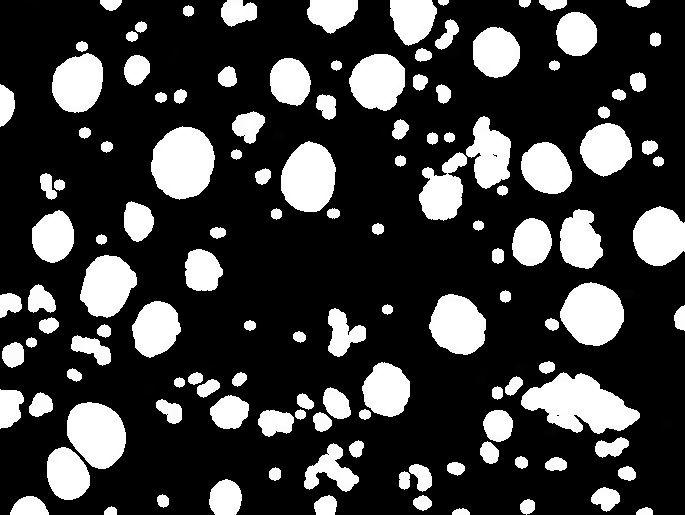
\includegraphics[width=\textwidth]{../code/task1/output/kernel_size_11.jpg}
    \captionof{figure}{\mintinline{python}{kernel_size = 11}}
\end{minipage}
\hfill
\begin{minipage}{0.24\textwidth}
    \centering
    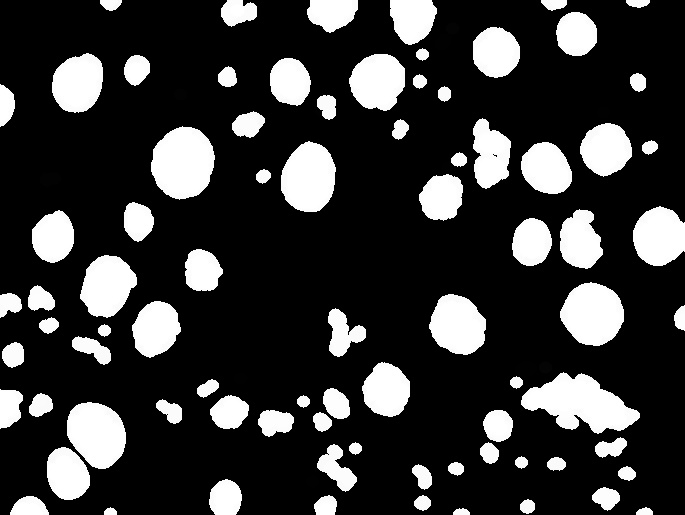
\includegraphics[width=\textwidth]{../code/task1/output/kernel_size_13.jpg}
    \captionof{figure}{\mintinline{python}{kernel_size = 13}}
\end{minipage}
\hfill
\begin{minipage}{0.24\textwidth}
    \centering
    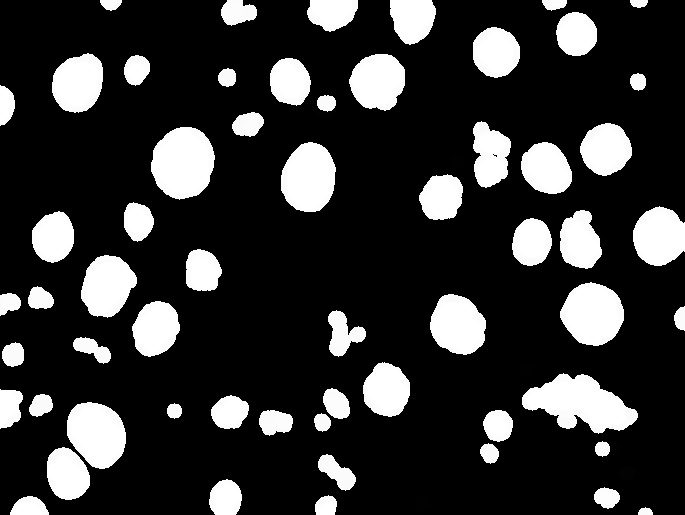
\includegraphics[width=\textwidth]{../code/task1/output/kernel_size_15.jpg}
    \captionof{figure}{\mintinline{python}{kernel_size = 15}}
\end{minipage}

\noindent
\begin{minipage}{0.24\textwidth}
    \centering
    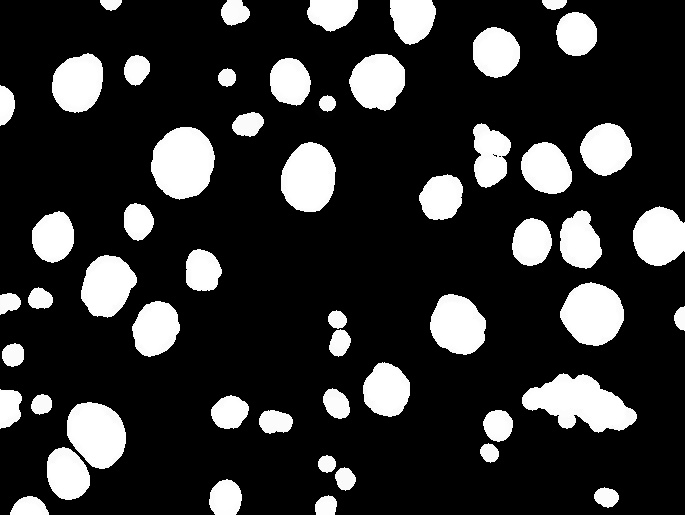
\includegraphics[width=\textwidth]{../code/task1/output/kernel_size_17.jpg}
    \captionof{figure}{\mintinline{python}{kernel_size = 17}}
\end{minipage}
\hfill
\begin{minipage}{0.24\textwidth}
    \centering
    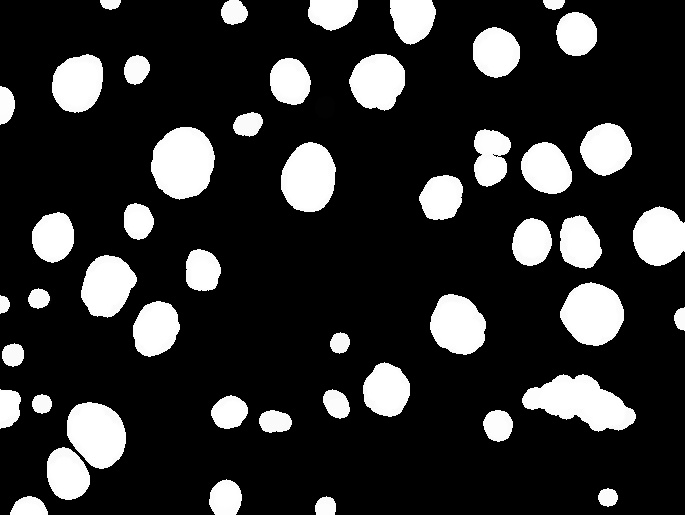
\includegraphics[width=\textwidth]{../code/task1/output/kernel_size_19.jpg}
    \captionof{figure}{\mintinline{python}{kernel_size = 19}}
\end{minipage}
\hfill
\begin{minipage}{0.24\textwidth}
    \centering
    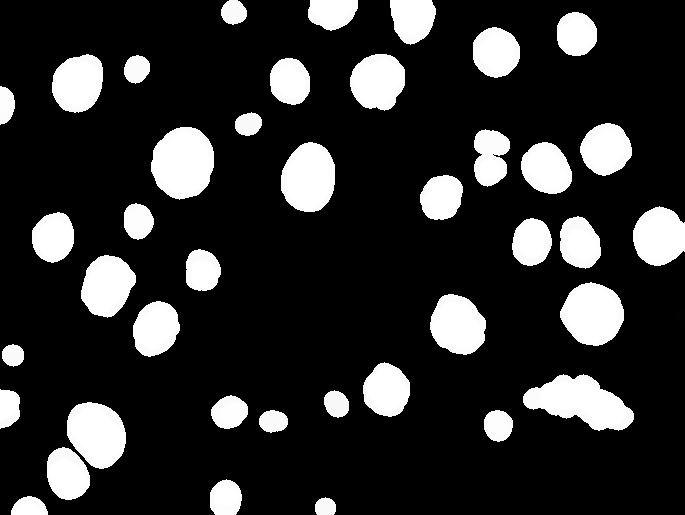
\includegraphics[width=\textwidth]{../code/task1/output/kernel_size_21.jpg}
    \captionof{figure}{\mintinline{python}{kernel_size = 21}}
\end{minipage}
\hfill
\begin{minipage}{0.24\textwidth}
    \centering
    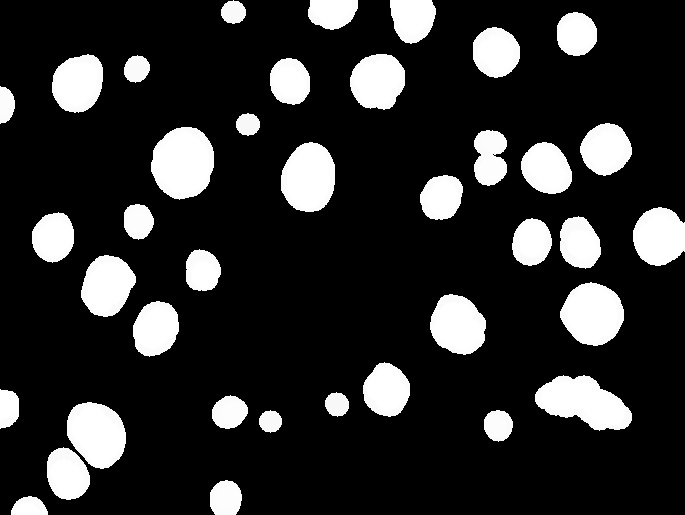
\includegraphics[width=\textwidth]{../code/task1/output/kernel_size_23.jpg}
    \captionof{figure}{\mintinline{python}{kernel_size = 23}}
\end{minipage}

\begin{minipage}{0.24\textwidth}
    \centering
    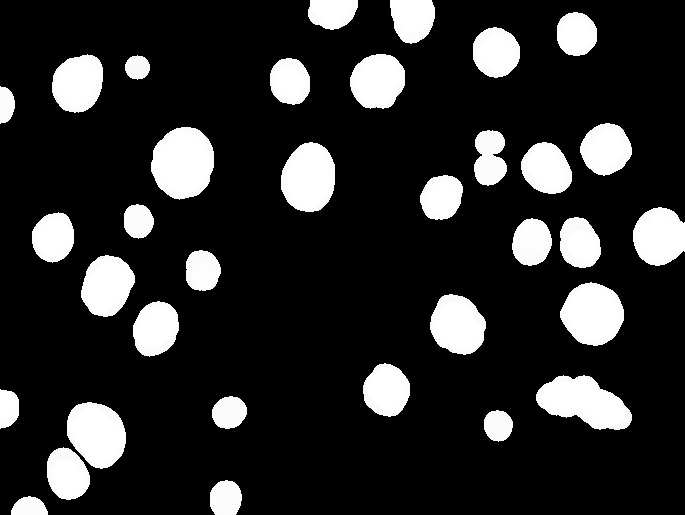
\includegraphics[width=\textwidth]{../code/task1/output/kernel_size_25.jpg}
    \captionof{figure}{\mintinline{python}{kernel_size = 25}}
\end{minipage}
\hfill
\begin{minipage}{0.24\textwidth}
    \centering
    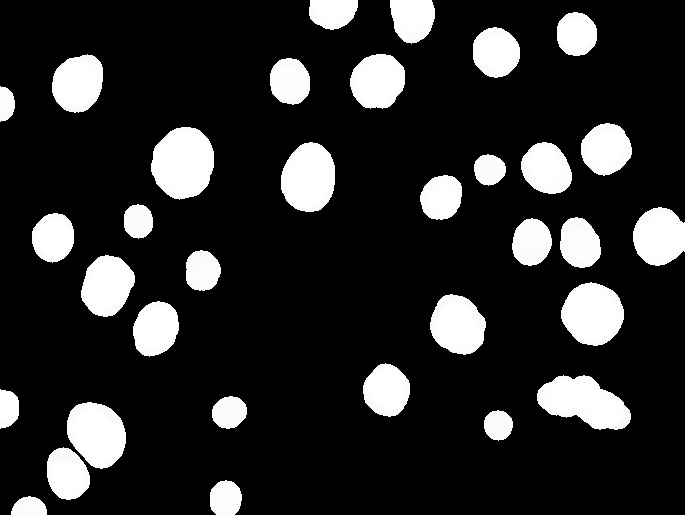
\includegraphics[width=\textwidth]{../code/task1/output/kernel_size_27.jpg}
    \captionof{figure}{\mintinline{python}{kernel_size = 27}}
\end{minipage}
\hfill
\begin{minipage}{0.24\textwidth}
    \centering
    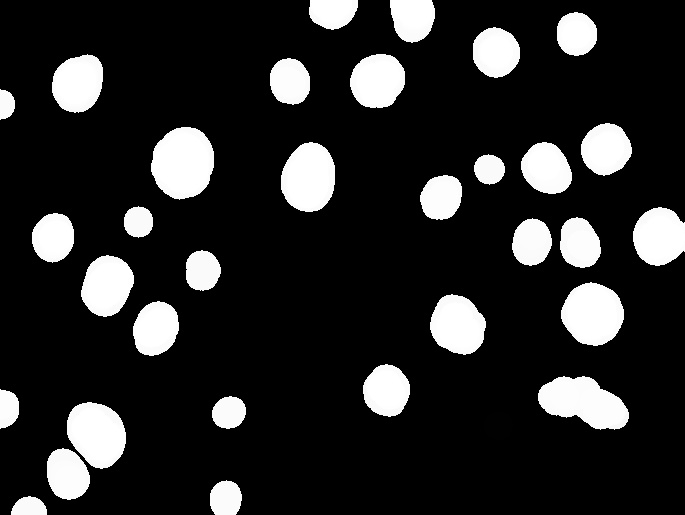
\includegraphics[width=\textwidth]{../code/task1/output/kernel_size_29.jpg}
    \captionof{figure}{\mintinline{python}{kernel_size = 29}}
\end{minipage}
\hfill
\begin{minipage}{0.24\textwidth}
    \centering
    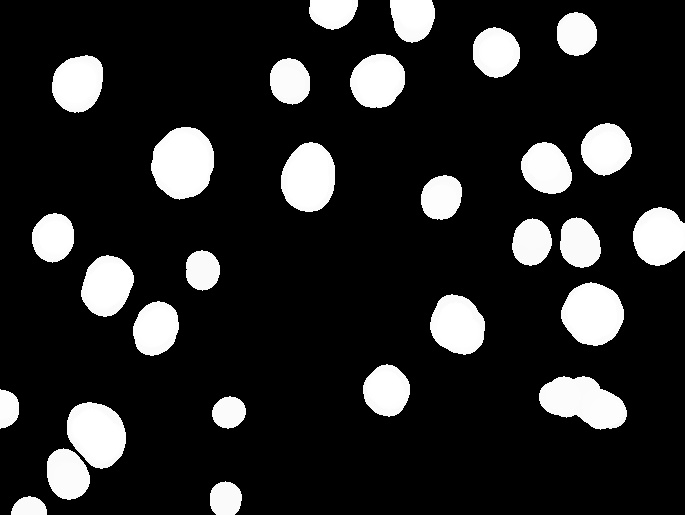
\includegraphics[width=\textwidth]{../code/task1/output/kernel_size_31.jpg}
    \captionof{figure}{\mintinline{python}{kernel_size = 31}}
\end{minipage}

I chose to open the image with a structuring element that had \mintinline{python}{kernel_size = 17} as it seemed to give the optimal balance between removing noise without significantly reducing the size of the remaining fat globules.

\begin{figure}[H]
    \centering
    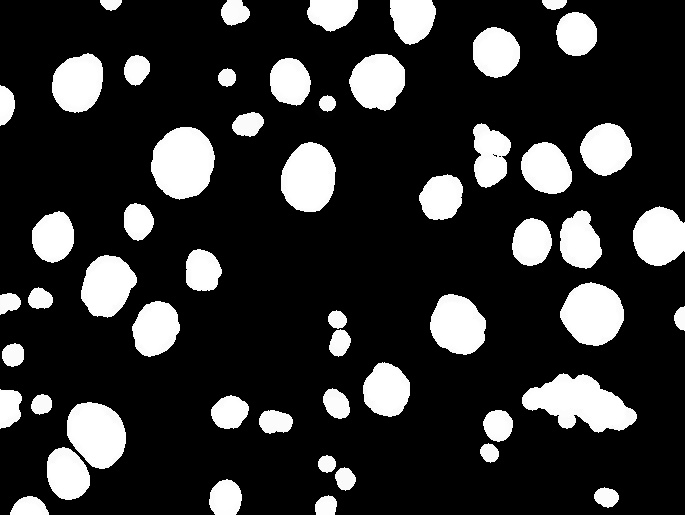
\includegraphics[width=0.5\textwidth]{../code/task1/output/kernel_size_17.jpg}
    \caption{Chosen noise threshold: \mintinline{python}{kernel_size = 17}}
\end{figure}

\subsection{Extraction of Binary Regions of Interest / Connected Components}
\begin{code}
\inputminted[firstline=1, lastline=9, linenos, breaklines, frame=single]{python}{../code/task1/5-7.py}
\caption{Task 1.5 section of \mintinline{python}{5-7.py}}
\end{code}

I'm not sure why, but no matter what level of noise removal I tried the connected components extraction with, the connected components always came out quite jagged.
To correct for this, I did some additional noise reduction by using a blur on the image to remove some of the white noise that was appearing in.
I also used a higher value of connectivity with \mintinline{python}{connectivity=8}, keeping components that were touching at all rather than components that just shared an edge.

\subsection{Filtering of Fat Globules}
\begin{code}
\inputminted[firstline=11, lastline=29, linenos, breaklines, frame=single]{python}{../code/task1/5-7.py}
\caption{Task 1.6 section of \mintinline{python}{5-7.py}}
\end{code}

I filtered the fat globules based off size \& compactness, using the compactness measure to remove globules that were not globule-shaped and the area measure to remove globules that were too small to be a globule.
I used a maximum compactness of 27 and a minimum area of 300 to filter the globules, resulting in a total of 35 fat globules.

\begin{figure}[H]
    \centering
    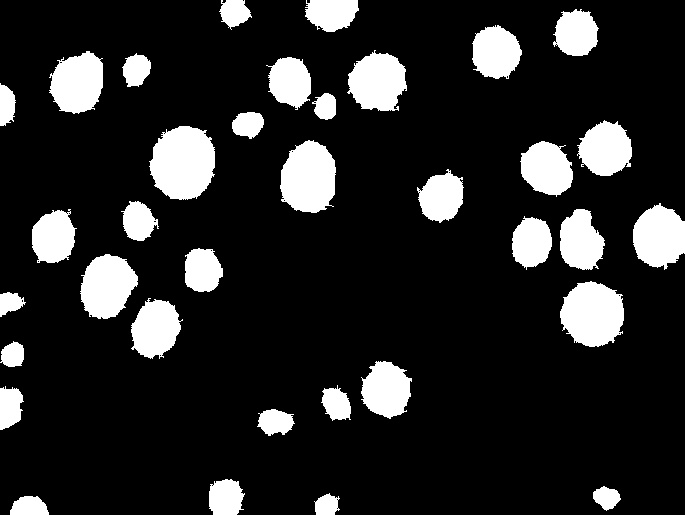
\includegraphics[width=0.5\textwidth]{../code/task1/output/filtered_fat_globules.jpg}
    \caption{Result of fat globule filtering}
\end{figure}

\subsection{Calculation of the Fat Area}
\begin{code}
\inputminted[firstline=31, lastline=40, linenos, breaklines, frame=single]{python}{../code/task1/5-7.py}
\caption{Task 1.7 section of \mintinline{python}{5-7.py}}
\end{code}

The percentage of the image covered by fat globules was 15.33\%.

\newpage


\section{Filtering of Images in Spatial \& Frequency Domains}
\begin{figure}[H]
    \centering
    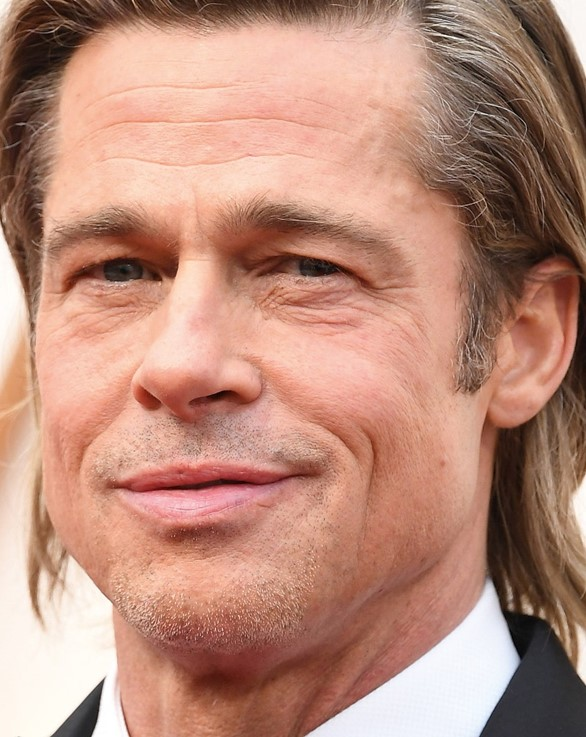
\includegraphics[width=0.5\textwidth]{../Task2.jpg}
    \caption{Original Facial Image}
\end{figure}

\subsection{Spatial Domain}
\begin{code}
\inputminted[firstline=5, lastline=13, linenos, breaklines, frame=single]{python}{../code/task2/task2.py}
\caption{Task 2.1 section of \mintinline{python}{task2.py}}
\end{code}

After some experimentation, I chose parameter values of \mintinline{python}{kernel_size = (15,15)} and \mintinline{python}{variance = 2} as, in my opinion, these yielded the best balance between blurring imperfections like wrinkles without causing the entire image to become too blurry.

\begin{figure}[H]
    \centering
    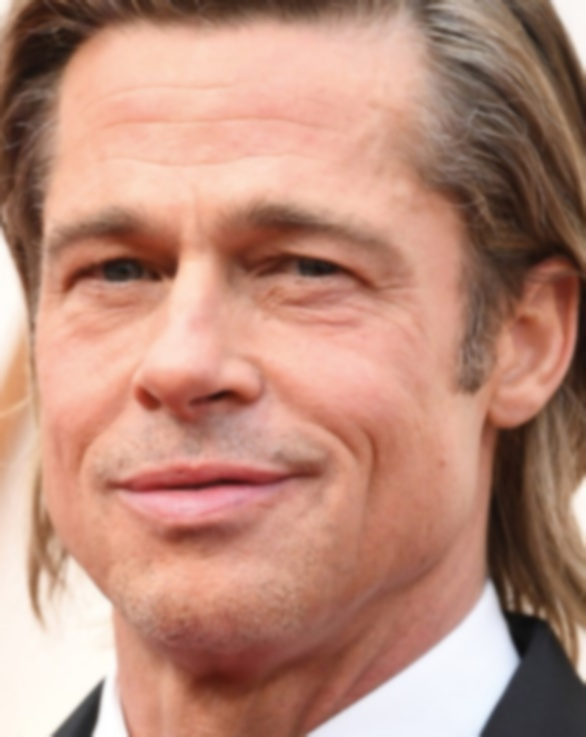
\includegraphics[width=0.5\textwidth]{../code/task2/output/1_spatial_domain.jpg}
    \caption{Output of \mintinline{python}{1_spatial_domain.jpg}}
\end{figure}

\subsection{Frequency Domain Low-Pass Filter}
\begin{code}
\inputminted[firstline=15, lastline=29, linenos, breaklines, frame=single]{python}{../code/task2/task2.py}
\caption{Task 2.2 section of \mintinline{python}{task2.py}}
\end{code}

\begin{figure}[H]
    \centering
    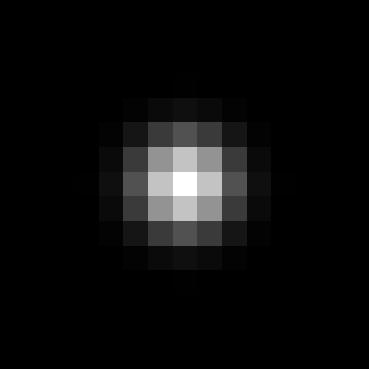
\includegraphics[width=0.5\textwidth]{../code/task2/output/2_frequency_domain_low-pass_filter.jpg}
    \caption{Zero-centered low-pass filter of Gaussian Kernel}
\end{figure}

\subsection{Frequency Domain Filtering}
\begin{code}
\inputminted[firstline=31, lastline=70, linenos, breaklines, frame=single]{python}{../code/task2/task2.py}
\caption{Task 2.3 section of \mintinline{python}{task2.py}}
\end{code}

\begin{figure}[H]
    \centering
    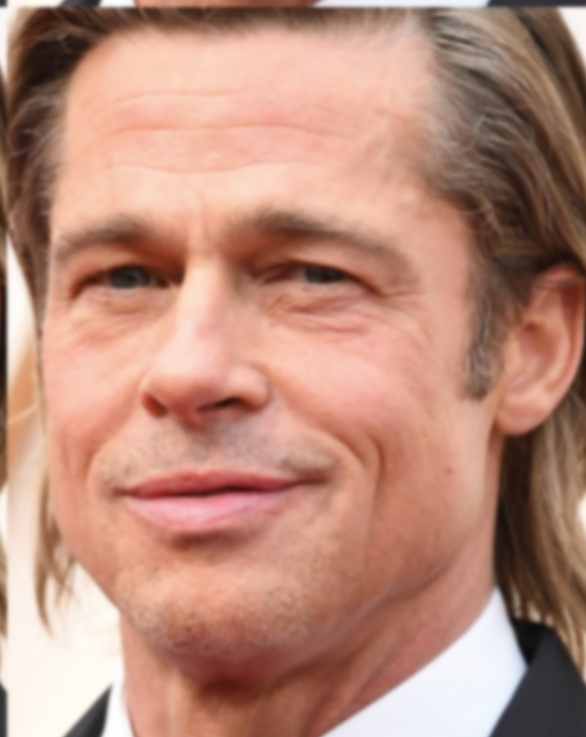
\includegraphics[width=0.5\textwidth]{../code/task2/output/3_filtered_color_image.jpg}
    \caption{Frequency domain filtered image}
\end{figure}

The low pass filter type used was the same as in Section 2.2: a Gaussian filter with \mintinline{python}{(15,15)} and \mintinline{python}{2}.

\subsection{Comparison}
\noindent
\begin{minipage}{0.49\textwidth}
\begin{figure}[H]
    \centering
    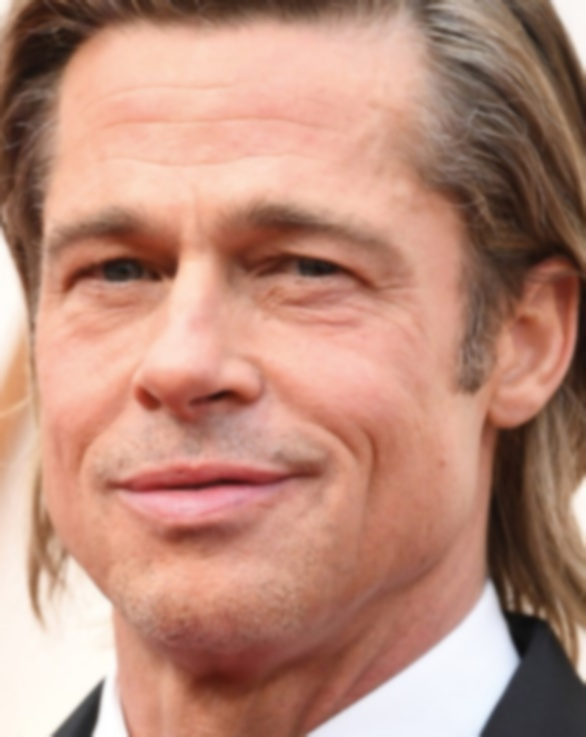
\includegraphics[width=\textwidth]{../code/task2/output/1_spatial_domain.jpg}
    \caption{Spatial domain filtered image}
\end{figure}
\end{minipage}
\hfill
\begin{minipage}{0.49\textwidth}
\begin{figure}[H]
    \centering
    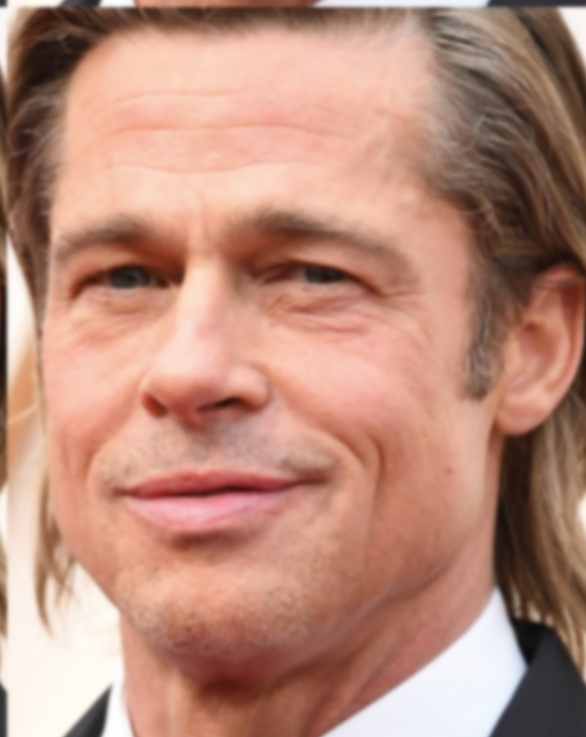
\includegraphics[width=\textwidth]{../code/task2/output/3_filtered_color_image.jpg}
    \caption{Frequency domain filtered image}
\end{figure}
\end{minipage}

The two images are very similar, having shared the same type of low pass filter.
However, the frequency domain filtered image has retained more colour range, and has an overall less blurred appearance.
The spatial domain filtering has applied a general blur across the entire image, making the filtering more obvious.
On the other hand, the frequency domain filtering is more subtle and reduces the visibility of wrinkles while retaining some definition in the eyes, lips, and stubble.
Overall, I would prefer the frequency domain filtering for this task; despite its increased complexity, it creates a more subtle and convincing effect that would be easily mistakable for an unfiltered image.

\subsection{Unseen Image Testing}
\noindent
\begin{minipage}{0.33\textwidth}
\begin{figure}[H]
    \centering
    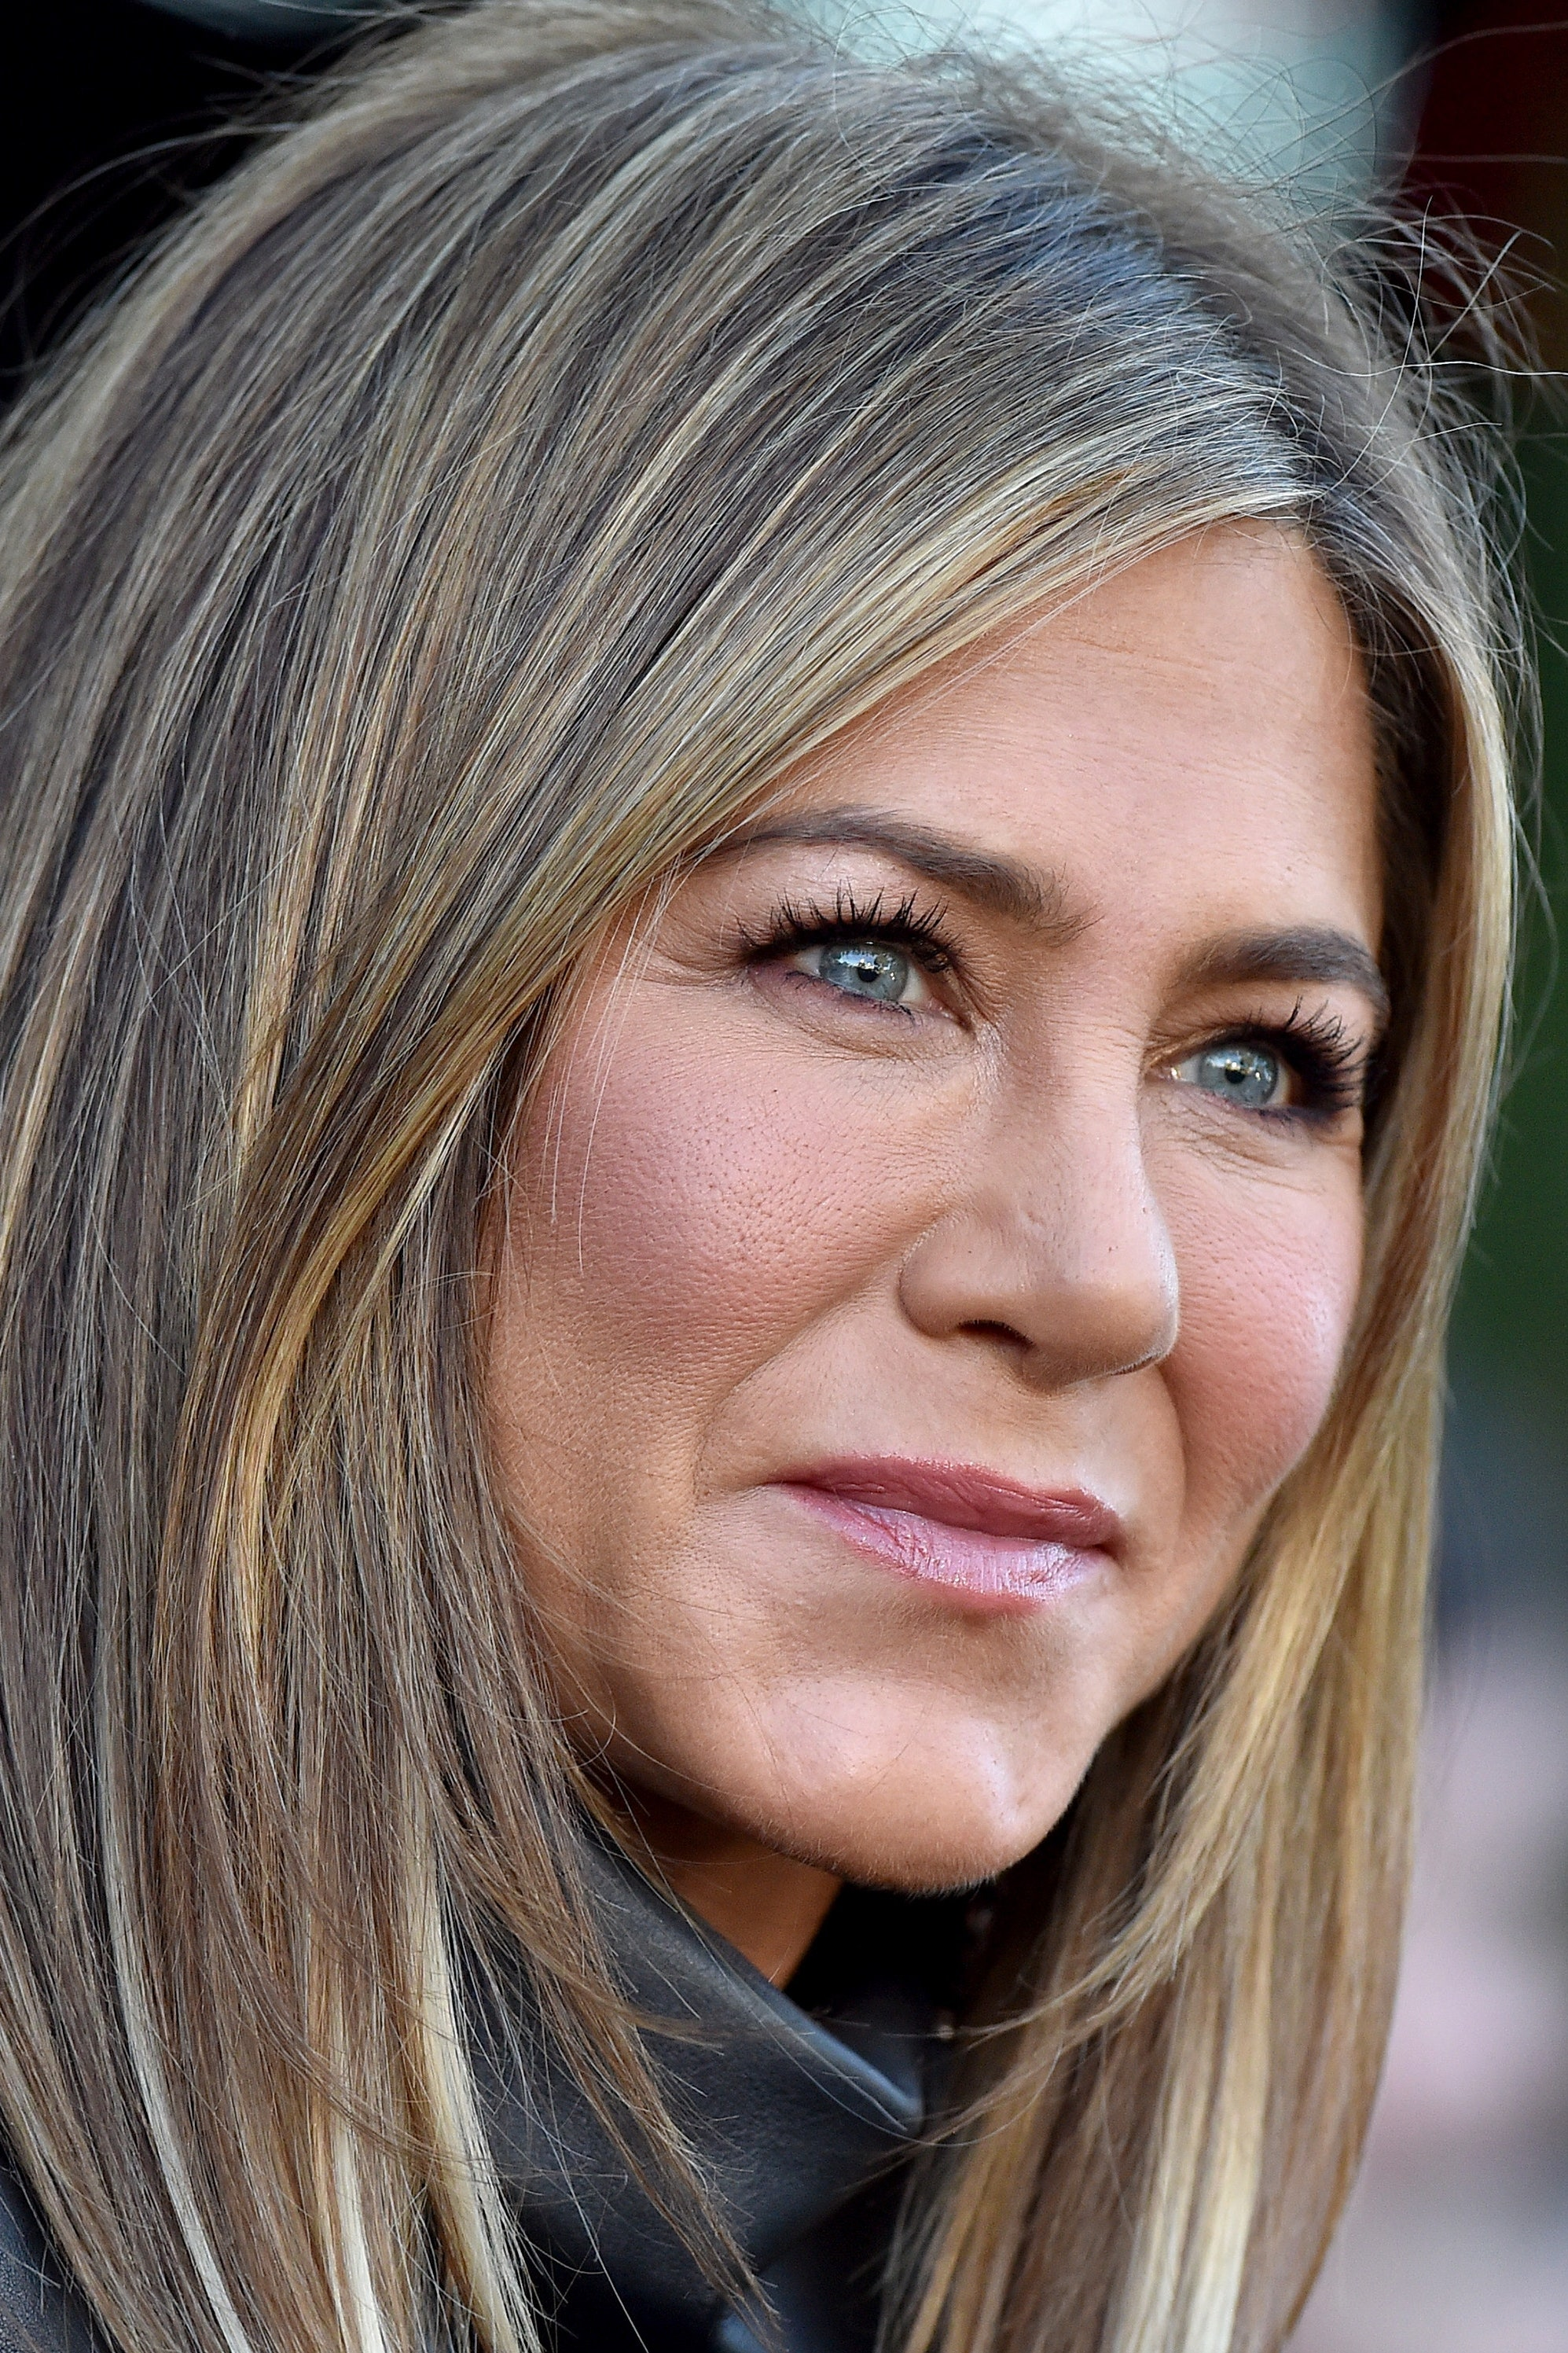
\includegraphics[width=\textwidth]{../code/task2/jennifer.jpg}
    \caption{Original Image}
\end{figure}
\end{minipage}
\hfill
\begin{minipage}{0.33\textwidth}
\begin{figure}[H]
    \centering
    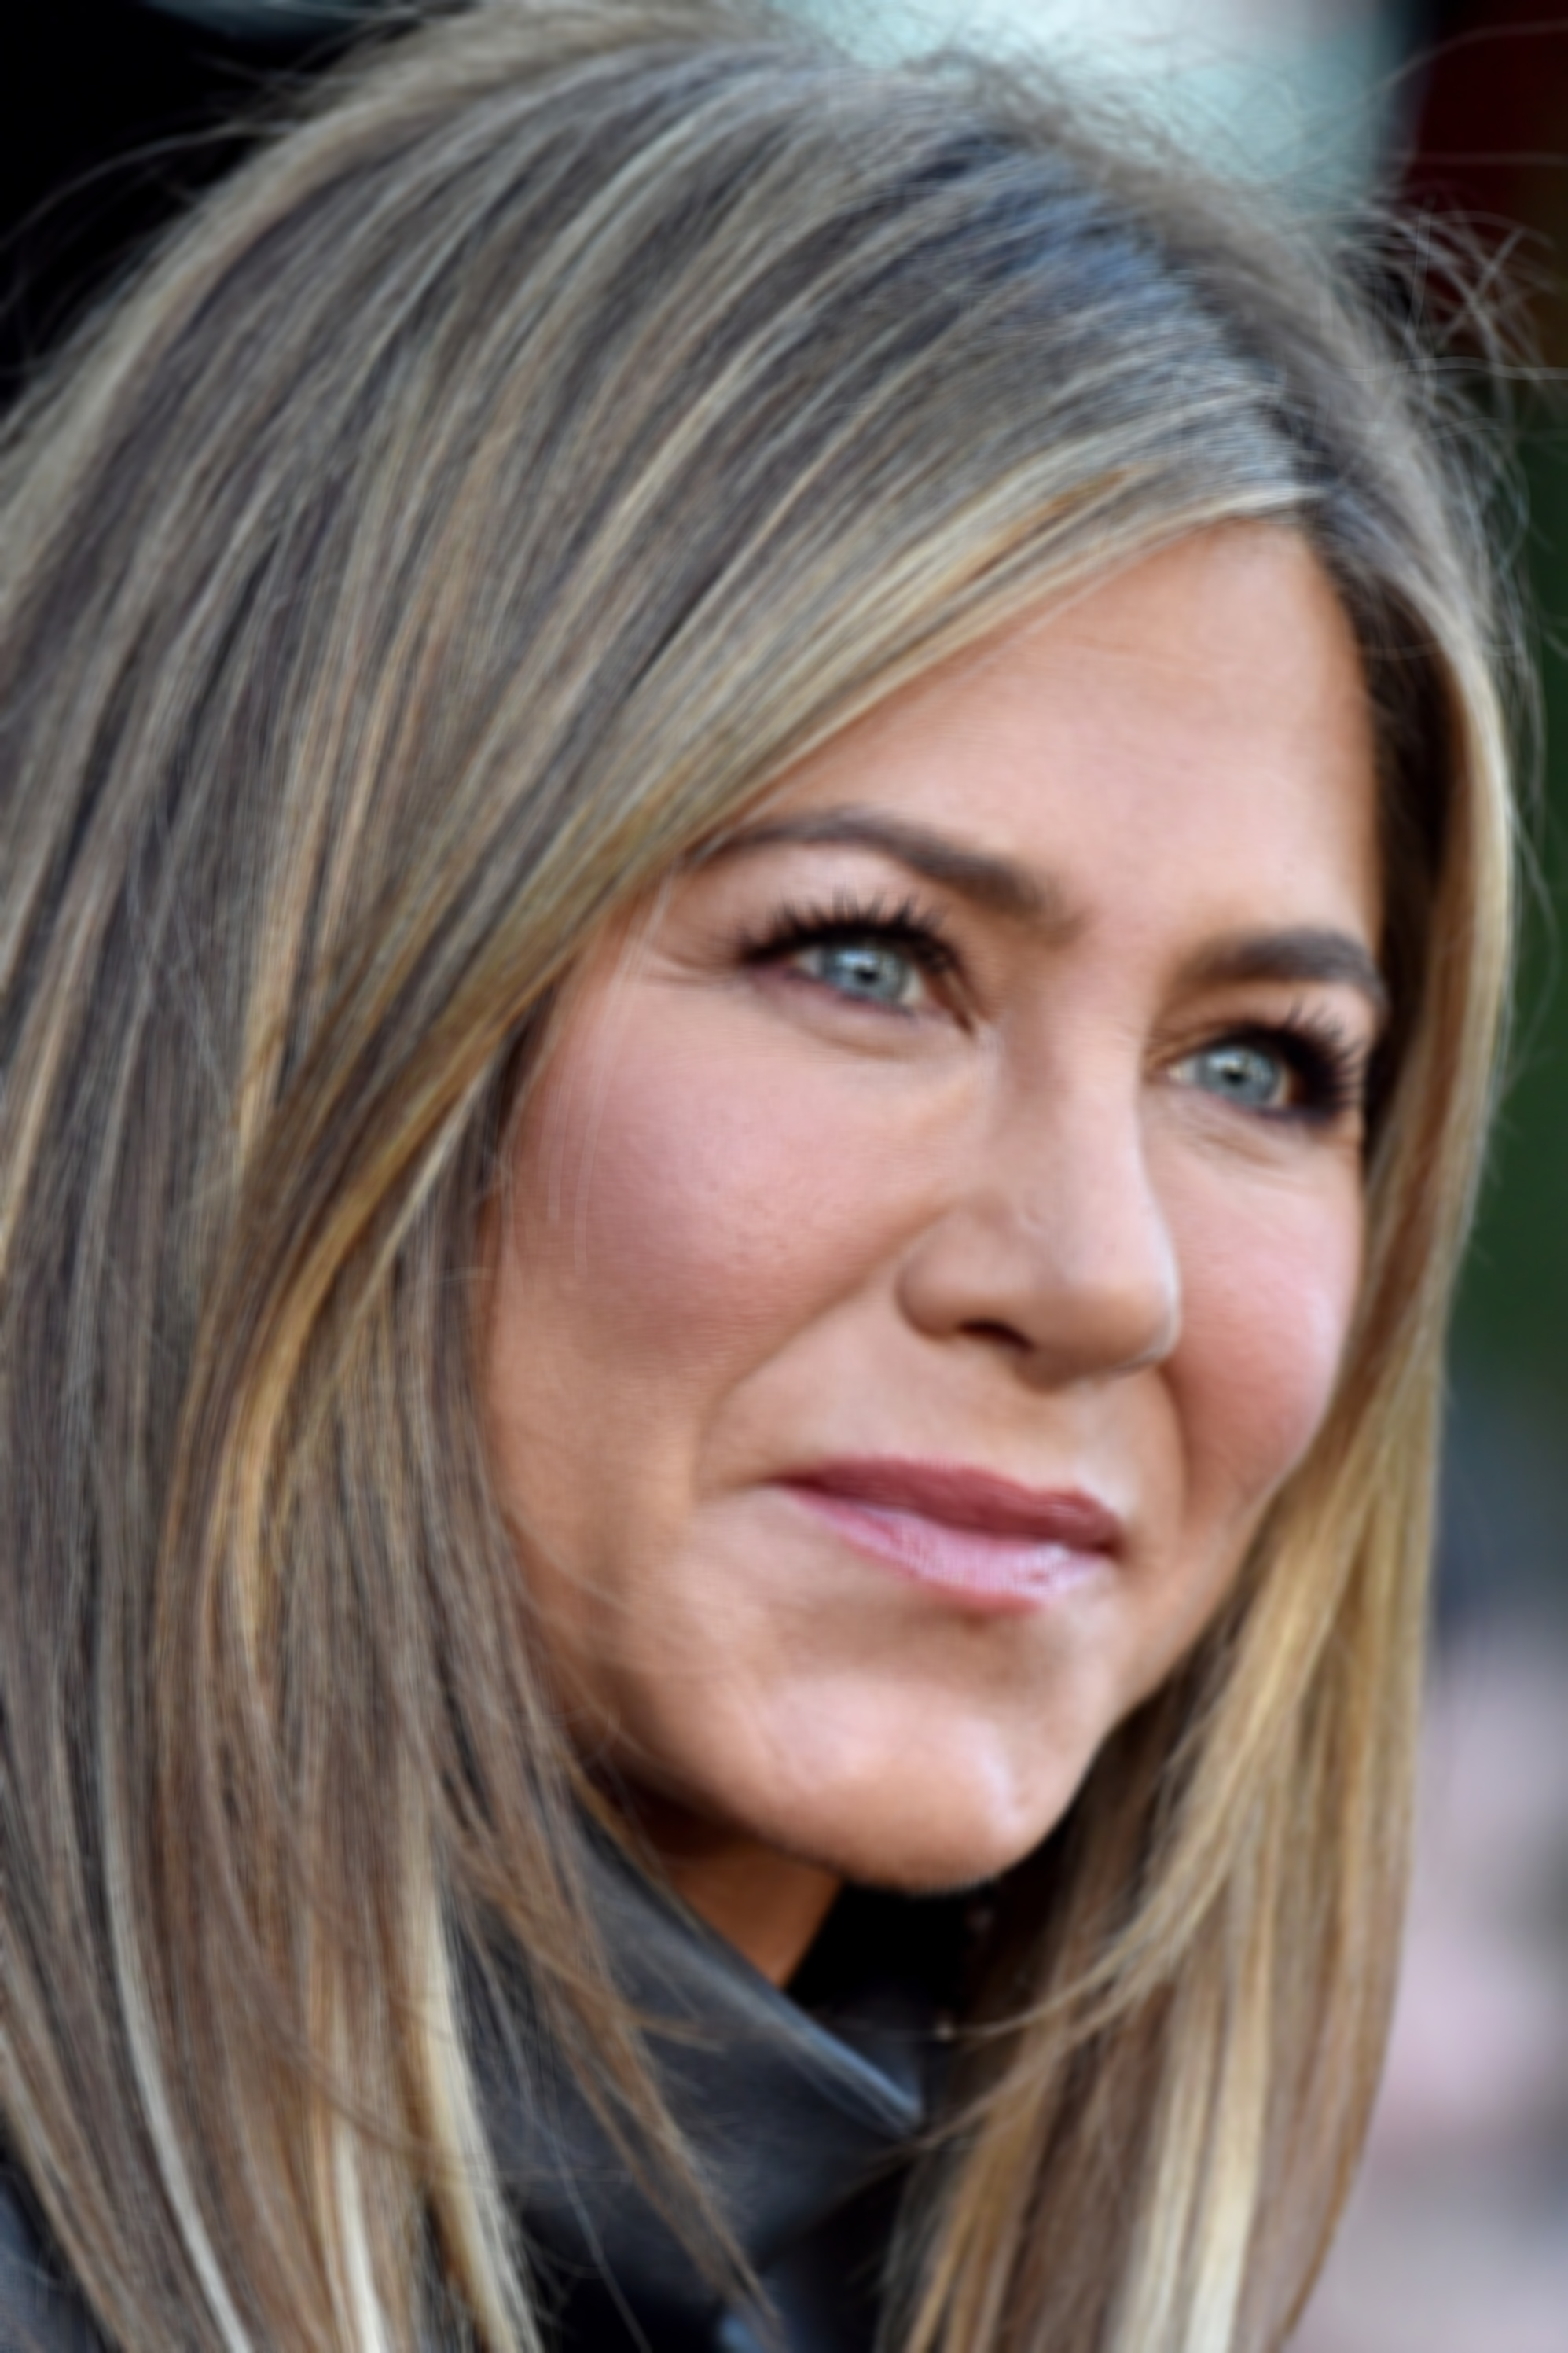
\includegraphics[width=\textwidth]{../code/task2/output/jennifer_spatial.jpg}
    \caption{Spatial domain filtered image}
\end{figure}
\end{minipage}
\hfill
\begin{minipage}{0.33\textwidth}
\begin{figure}[H]
    \centering
    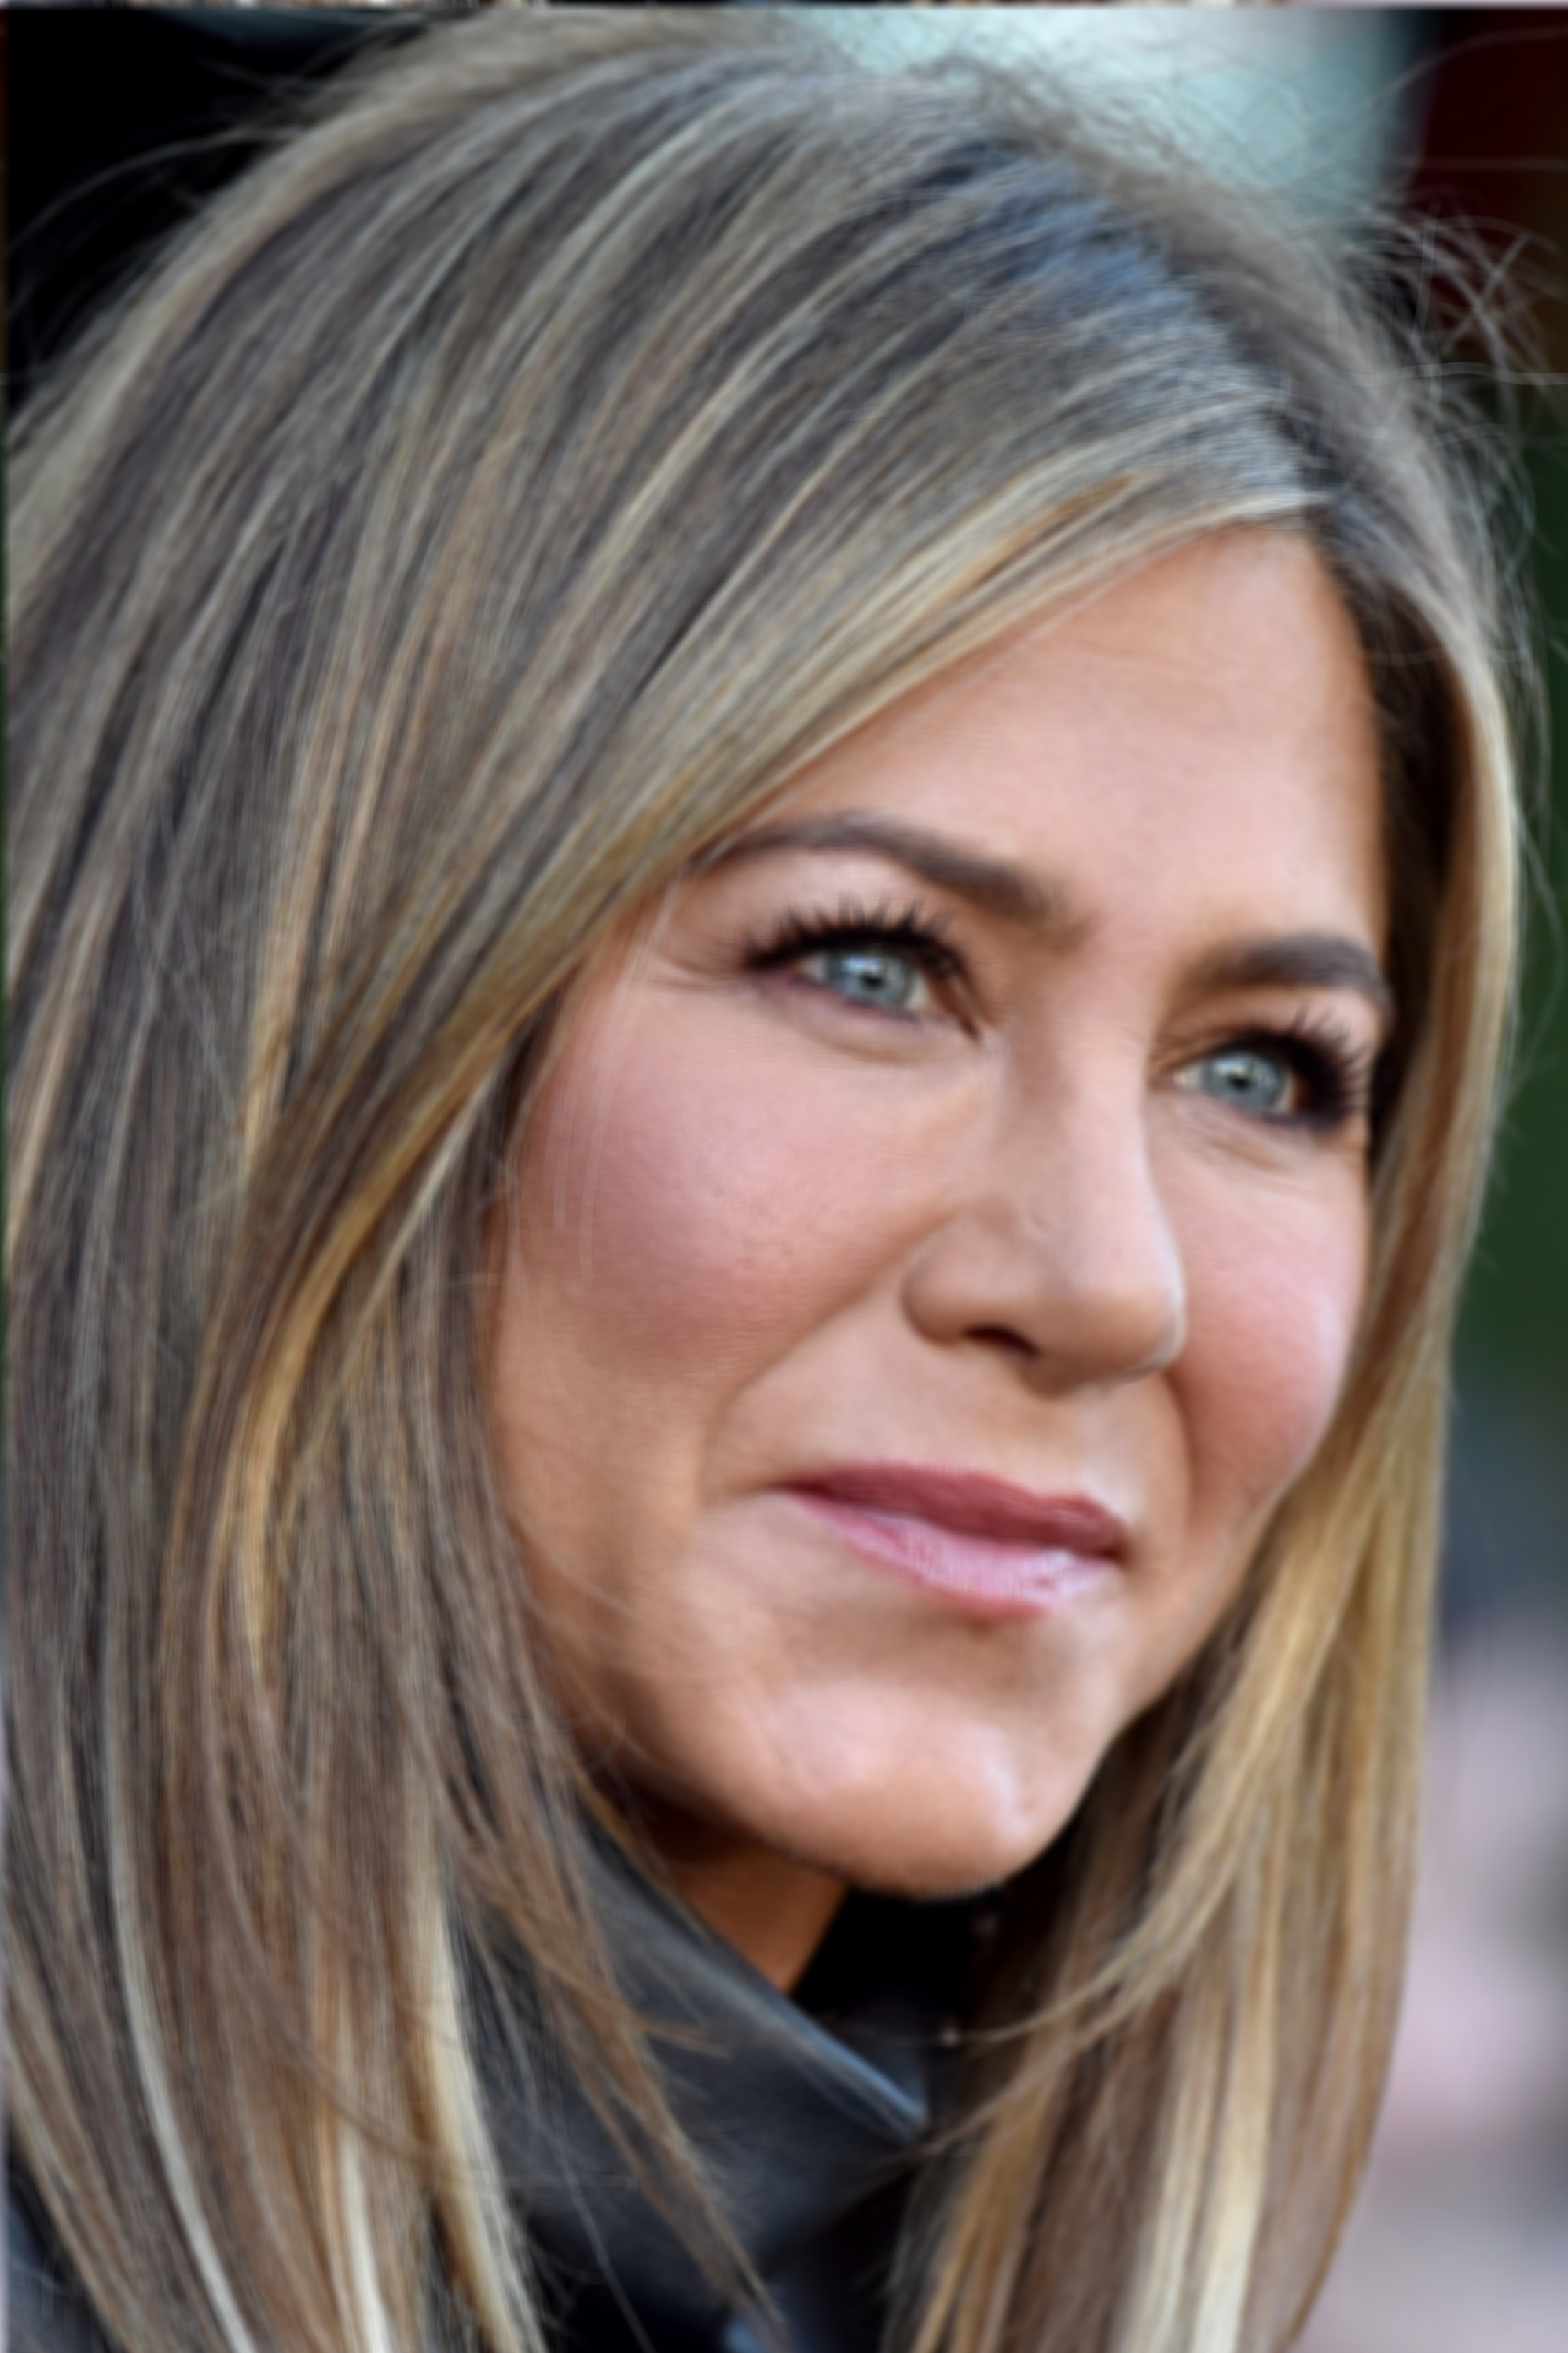
\includegraphics[width=\textwidth]{../code/task2/output/jennifer_freq.jpg}
    \caption{Frequency domain filtered}
\end{figure}
\end{minipage}

Again, the two filtered images are very similar.
In my opinion, the frequency domain filtered image performed better here again, as it has a more dynamic colour range and more subtle blurring.
The skin looks very artificially smoothed in the spatial domain filtered image, but more natural in the frequency domain filtered image.
The hair looks more blurred and out-of-focus in the spatial domain filtered image, but looks sharper and more natural in the frequency domain filtered image.

\end{document}
